\Hefteintrag{1.9}{Darstellung von m:n-Beziehungen}{

m:n-Beziehungen können im UML-Klassendiagramm auf zwei verschiedene Arten dargestellt werden:
\vspace{0.5cm}

\emphColA{1. \LoesungLuecke{als direkte Beziehung}{15cm}}\\
Vorteil: \LoesungLuecke{Diagramm kompakt und übersichtlich}{15cm}

\vspace{0.5cm}
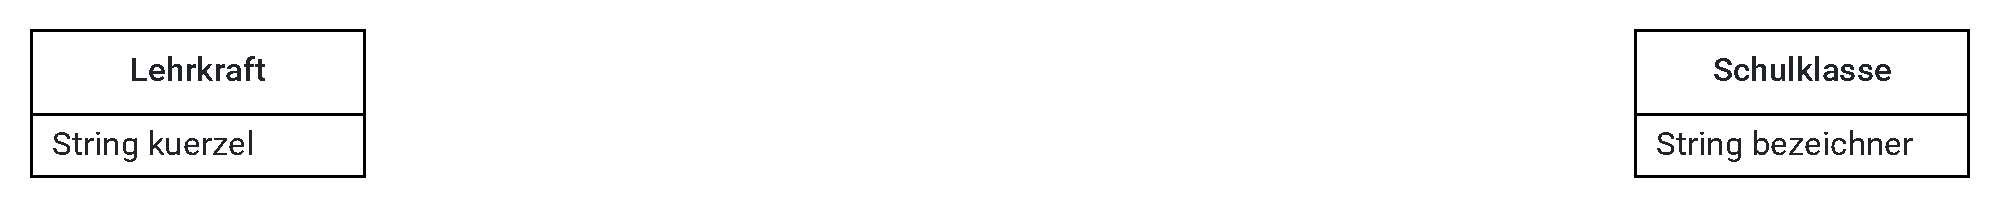
\includegraphics[width=\textwidth]{img/mn-Beispiel}


\emphColA{2. \LoesungLuecke{mit Beziehungstabelle}{15cm}}\\
Vorteil: \LoesungLuecke{Diagramm kompakt und übersichtlich}{15cm}

\vspace{1.5cm}
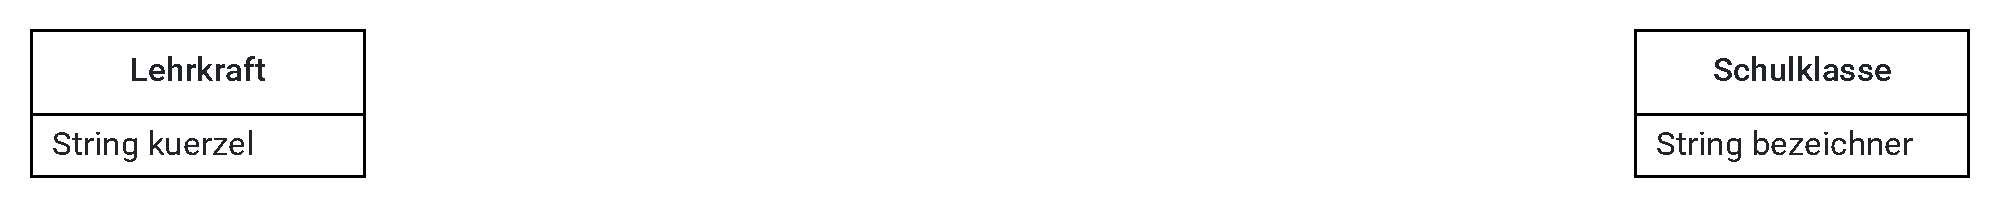
\includegraphics[width=\textwidth]{img/mn-Beispiel}\\

}